\usepackage[margin=1in]{geometry}
\usepackage{amsmath,amssymb,amsthm,mathtools}
\usepackage{array}
\usepackage{enumitem}
\usepackage{hyperref}
\usepackage{tikz}
\usetikzlibrary{arrows.meta,calc,positioning,decorations.markings,
  decorations.pathmorphing,patterns,shadings,shapes.geometric,fadings,
  backgrounds,intersections,bending}
\usepackage{thmtools}
\usepackage{cleveref}

% Monochrome palette for classic textbook-style figures.  The imported TikZ
% figures use these semantic color names; mapping them to black/gray removes
% color while preserving line weights, fills, and diagram structure.
\definecolor{formteal}{gray}{0.00}
\definecolor{formgold}{gray}{0.00}
\definecolor{formrust}{gray}{0.00}
\definecolor{formplum}{gray}{0.00}
\definecolor{formsage}{gray}{0.00}
\definecolor{formslate}{gray}{0.00}
\definecolor{formivory}{gray}{1.00}

\newcommand{\sagedir}{../sagemath}
\input{\sagedir/coords.tex}
\input{\sagedir/coords_torus.tex}
\input{\sagedir/coords_curve_sample.tex}

\newcommand{\drawprecisetorus}{%
  \fill[formteal!13, line join=round] plot[smooth cycle] coordinates {\torusOuter};
  \fill[white, line join=round] plot[smooth cycle] coordinates {\torusInner};
  \foreach \name in {Zero,One,Two,Three,Four,Five,Six,Seven}{%
    \draw[draw=formteal!60!black, line width=0.42pt, line join=round, opacity=0.9]
      plot[smooth] coordinates {\csname torusMer\name VA\endcsname};}
  \draw[draw=formteal!60!black, line width=0.42pt, line join=round, opacity=0.9]
    plot[smooth] coordinates {\torusMerFiveVB};
  \draw[draw=formteal!60!black, line width=0.42pt, line join=round, opacity=0.9]
    plot[smooth] coordinates {\torusMerSixVB};
  \draw[draw=formteal!60!black, line width=0.42pt, line join=round, opacity=0.9]
    plot[smooth] coordinates {\torusMerSevenVB};
  \draw[draw=formteal!60!black, line width=0.5pt, line join=round, opacity=0.95]
    plot[smooth] coordinates {\torusLonTopVA};
  \draw[draw=formteal!60!black, line width=0.42pt, line join=round, opacity=0.8]
    plot[smooth] coordinates {\torusLonOuterVA};
  \draw[draw=formteal!60!black, line width=0.42pt, line join=round, opacity=0.8]
    plot[smooth] coordinates {\torusLonInnerVA};
  \draw[draw=formteal!65!black, line width=0.95pt, line join=round]
    plot[smooth cycle] coordinates {\torusOuter};
  \draw[draw=formteal!65!black, line width=0.8pt, line join=round]
    plot[smooth cycle] coordinates {\torusInner};
}

\newcommand{\drawprecisecurve}{%
  \draw[draw=formteal!60!black, line width=0.88pt, line join=round]
    plot[smooth cycle, tension=0.85] coordinates {\curveOvalFull};
  \draw[draw=formteal!60!black, line width=0.88pt, line join=round]
    plot[smooth, tension=0.9] coordinates {\curveBranchUpper};
  \draw[draw=formteal!60!black, line width=0.88pt, line join=round]
    plot[smooth, tension=0.9] coordinates {\curveBranchLower};
  \fill[formteal!70!black] (-1,0) circle (1.8pt);
  \fill[formteal!70!black] ( 0,0) circle (1.8pt);
  \fill[formteal!70!black] ( 1,0) circle (1.8pt);
}

\newcommand{\classicTrinityDiagram}{%
  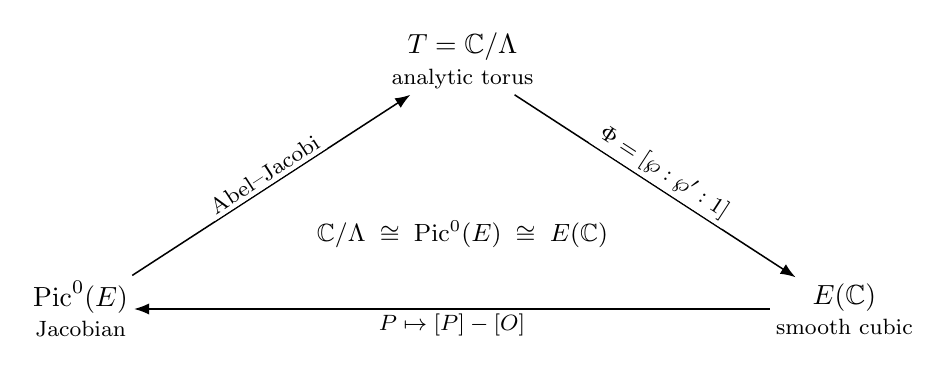
\begin{tikzpicture}[>=Latex,
      object/.style={align=center, inner sep=2pt},
      map/.style={->, line width=0.55pt},
      lab/.style={font=\footnotesize, fill=white, inner sep=1.5pt}]
    \node[object] (T) at (0,3.15)
      {$T=\C/\Lambda$\\[-1pt]{\footnotesize analytic torus}};
    \node[object] (E) at (4.85,0)
      {$E(\C)$\\[-1pt]{\footnotesize smooth cubic}};
    \node[object] (J) at (-4.85,0)
      {$\Pic^0(E)$\\[-1pt]{\footnotesize Jacobian}};
    \draw[map] (T) -- node[lab, sloped, above] {$\Phi=[\wp:\wp':1]$} (E);
    \draw[map] (E) -- node[lab, below] {$P\mapsto [P]-[O]$} (J);
    \draw[map] (J) -- node[lab, sloped, above] {Abel--Jacobi} (T);
    \node[font=\small] at (0,0.95)
      {$\C/\Lambda\;\cong\;\Pic^0(E)\;\cong\;E(\C)$};
  \end{tikzpicture}%
}

\newcommand{\classicChordDiagram}{%
  \begin{tikzpicture}[scale=1.0, every node/.style={font=\small}]
    \draw[->, black!55, line width=0.45pt] (-1.7,0) -- (2.7,0) node[right] {$x$};
    \draw[->, black!55, line width=0.45pt] (0,-3.3) -- (0,3.5) node[above] {$y$};
    \drawprecisecurve
    \draw[black, line width=0.65pt]
      (\chordlefta,\chordleftb) -- (\chordrighta,\chordrightb);
    \draw[dashed, black!65, line width=0.45pt]
      (\chordRx,\chordRy) -- (\chordSx,\chordSy);
    \fill[black] (\chordPx,\chordPy) circle (2.1pt);
    \node[above left] at (\chordPx,\chordPy) {$P$};
    \fill[black] (\chordQx,\chordQy) circle (2.1pt);
    \node[above right] at (\chordQx,\chordQy) {$Q$};
    \fill[black] (\chordRx,\chordRy) circle (2.1pt);
    \node[above left] at (\chordRx,\chordRy) {$R$};
    \fill[black] (\chordSx,\chordSy) circle (2.3pt);
    \node[below left] at (\chordSx,\chordSy) {$P\oplus Q=-R$};
  \end{tikzpicture}%
}

\newcommand{\classicExpSequenceDiagram}{%
  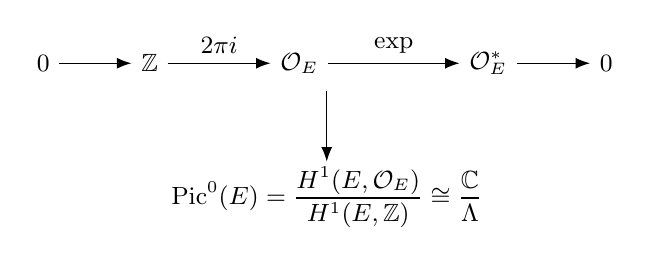
\begin{tikzpicture}[>=Latex, every node/.style={font=\small}]
    \node (z0) at (0,0) {$0$};
    \node (Z) at (1.35,0) {$\Z$};
    \node (O) at (3.25,0) {$\OO_E$};
    \node (Os) at (5.65,0) {$\OO_E^*$};
    \node (z1) at (7.15,0) {$0$};
    \draw[->, line width=0.5pt] (z0)--(Z);
    \draw[->, line width=0.5pt] (Z)--node[above] {$2\pi i$} (O);
    \draw[->, line width=0.5pt] (O)--node[above] {$\exp$} (Os);
    \draw[->, line width=0.5pt] (Os)--(z1);
    \draw[->, line width=0.5pt] (3.6,-0.35) -- (3.6,-1.25);
    \node[align=center] at (3.6,-1.7)
      {$\displaystyle \Pic^0(E)
        =\frac{H^1(E,\OO_E)}{H^1(E,\Z)}
        \cong \frac{\C}{\Lambda}$};
  \end{tikzpicture}%
}

\setlist[enumerate]{leftmargin=*, itemsep=0.35em}
\setlist[itemize]{leftmargin=*, itemsep=0.25em}
\allowdisplaybreaks
\emergencystretch=2em
\newcolumntype{L}[1]{>{\raggedright\arraybackslash}p{#1}}

\newcommand{\C}{\mathbb{C}}
\newcommand{\R}{\mathbb{R}}
\newcommand{\Z}{\mathbb{Z}}
\newcommand{\Q}{\mathbb{Q}}
\newcommand{\F}{\mathbb{F}}
\newcommand{\CP}{\mathbb{CP}}
\newcommand{\HH}{\mathbb{H}}
\newcommand{\OO}{\mathcal{O}}
\newcommand{\M}{\mathcal{M}}
\newcommand{\Div}{\operatorname{Div}}
\newcommand{\Pic}{\operatorname{Pic}}
\newcommand{\Prin}{\operatorname{Prin}}
\newcommand{\Jac}{\operatorname{Jac}}
\newcommand{\Gal}{\operatorname{Gal}}
\newcommand{\GL}{\operatorname{GL}}
\newcommand{\SL}{\operatorname{SL}}
\newcommand{\Span}{\operatorname{span}}
\newcommand{\divisor}{\operatorname{div}}
\newcommand{\ord}{\operatorname{ord}}
\newcommand{\Res}{\operatorname{Res}}
\newcommand{\degdiv}{\operatorname{deg}}
\newcommand{\rank}{\operatorname{rank}}
\newcommand{\dd}{\,d}
\newcommand{\wpprime}{\wp'}
\newcommand{\smap}{\mathfrak{s}}
\newcommand{\tate}{T_\ell E}

\declaretheorem[name=Theorem,numberwithin=chapter]{theorem}
\declaretheorem[name=Proposition,sibling=theorem]{proposition}
\declaretheorem[name=Lemma,sibling=theorem]{lemma}
\declaretheorem[name=Corollary,sibling=theorem]{corollary}
\declaretheorem[name=Definition,sibling=theorem,style=definition]{definition}
\declaretheorem[name=Example,sibling=theorem,style=definition]{example}
\declaretheorem[name=Remark,sibling=theorem,style=remark]{remark}
\declaretheorem[name=Warning,sibling=theorem,style=remark]{warningthm}
\let\warning\warningthm
\let\endwarning\endwarningthm
\declaretheorem[name=Exercise,numberwithin=chapter,style=definition]{exercise}

\newcommand{\exerciseintent}[1]{%
  \par\smallskip
  \noindent{\footnotesize\color{black!55}\emph{Intent.} #1\par}
  \smallskip
}

\newenvironment{keyidea}[1]{%
  \par\medskip
  \begin{center}
  \begin{minipage}{0.92\textwidth}
  \hrule
  \smallskip
  \textbf{#1.}\quad\ignorespaces
}{%
  \smallskip
  \hrule
  \end{minipage}
  \end{center}
  \medskip
}

\tikzset{
  arrow/.style={-{Latex[length=2mm]}, thick},
  point/.style={circle, fill=black, inner sep=1.5pt},
  labelnode/.style={font=\small, align=center},
  note/.style={draw=black!55, rounded corners=2pt, align=center, inner sep=5pt, fill=black!3},
  visualnode/.style={draw=black!60, rounded corners=2pt, align=center, inner sep=6pt, fill=black!2},
  smallvisual/.style={draw=black!60, rounded corners=2pt, align=center, inner sep=4pt, fill=black!2}
}

\crefname{warningthm}{warning}{warnings}
\Crefname{warningthm}{Warning}{Warnings}
\crefname{exercise}{exercise}{exercises}
\Crefname{exercise}{Exercise}{Exercises}
